
\subsection{Convergence analysis}

We test our code on the problem 

\begin{align}
f_x = \frac{E}{1-\nu^2} (-2y^2 - x^2 + \nu x^2 - 2\nu xy -2xy + 3 - \nu) \\
f_y = \frac{E}{1-\nu^2} (-2x^2 - y^2 + \nu y^2 - 2\nu xy -2xy + 3 - \nu) 
\end{align}

with homogeneous Dirichlet boundary conditions on all boundaries. Compared to the analytical solution 

\begin{align}
\bm{u}(x,y) = \begin{bmatrix}
\, (x^2-1)(y^2-1) \, \\
(x^2-1)(y^2-1)
\end{bmatrix}
\end{align}

we get the error plot shown in Figure \ref{error}. Also, increasing the grid size in each spatial direction by a factor 2, we obtain an accuracy convergence of order 2, as shown in Figure \ref{convergence}. This implies that our code is correct.

\begin{figure}
\center
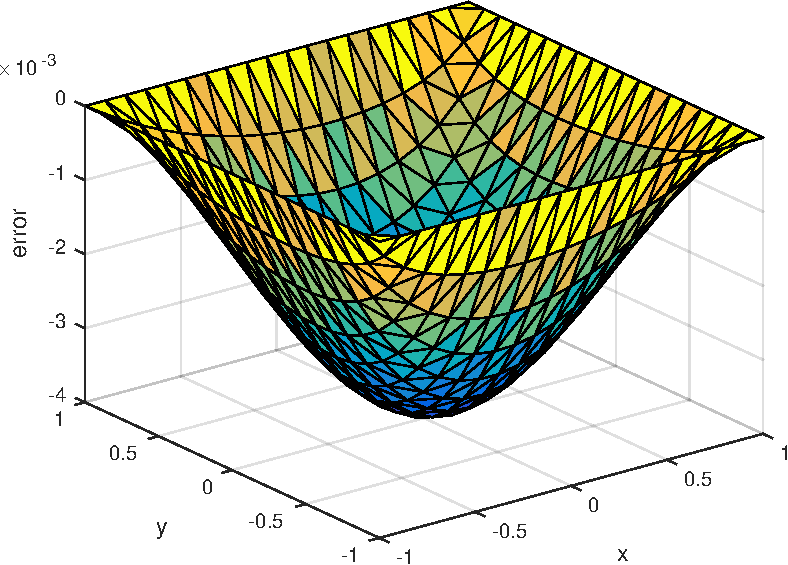
\includegraphics[scale=0.5]{error_linEl}
\caption{Error between the numerical solution to the linear elasticity problem and the analytical solution with $N = 20$ grid points in each spatial direction. The numerical solution is smaller than the analytical solution.}
\label{error}
\end{figure}

\begin{figure}[ht]
\center
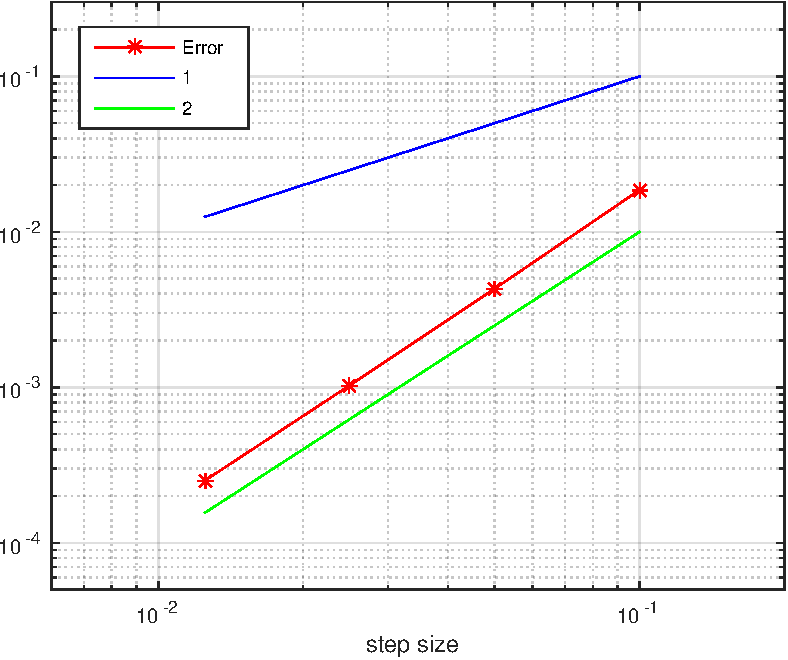
\includegraphics[scale=0.5]{conv_linEl}
\caption{Loglog plot of the error showing convergence of order 2 of the linear elasticity problem with $N =$ 10, 20, 40 and 80 grid points in each spatial direction. }
\label{convergence}
\end{figure}

